\documentclass[12pt,a4paper]{article}%
\usepackage{makeidx}
\makeindex
\usepackage{bm}
\usepackage{framed} % Easier way to use Framebox
\usepackage{pdfpages} % Import PDF in latex document
\usepackage{listings}
\usepackage{array}
\usepackage{enumitem}
\usepackage{amsmath, amssymb, amsthm}  % For mathematical symbols
\usepackage{colortbl,color}
\usepackage{xcolor}
\usepackage{auto-pst-pdf}
\usepackage{graphicx,psfrag}
\usepackage{tabularx,array}
\usepackage{booktabs}
\usepackage{multirow}
\usepackage{multicol}
\usepackage[subfigure]{tocloft}
\usepackage[tight]{subfigure}
\usepackage{float,booktabs,threeparttable}
\usepackage{caption}
\usepackage{mathtools} % add text on arrows
\usepackage{longtable}
\usepackage{appendix}
\usepackage{pdfpages}
\usepackage{blkarray} %For adding Matrix label on row and column
\usepackage{url}
\usepackage{indentfirst} % indent the first paragraph of new section
\usepackage{titlesec} % change the way \subsubsubsection formats
\usepackage{mathtools} % for pre-superscript and pre-subscript on notation

\def\se{{\rm se}}
%\newcommand{\red}{\color{red}}
\linespread{1.5}  % The linespread is 1.5.

% Numbered theorems, definitions, algorithm and lemmas ======================================================================
\newtheorem{thm}{Theorem}  % Define new theorem.
\newtheorem{alg}{Algorithm}[section]  % Define new algorithm.
\newtheorem{definition}{Definition}
% ===========================================================================================================================

% For writing pseudo code ======================================================================
\usepackage{algorithm}% http://ctan.org/pkg/algorithms
\usepackage{algpseudocode}% http://ctan.org/pkg/algorithmicx
% ===========================================================================================================================

\theoremstyle{definition}
\theoremstyle{plain}
\setcounter{secnumdepth}{5}


\renewcommand{\contentsname}{Table of Contents}
\renewcommand{\listfigurename}{List of Figures}
\renewcommand{\listtablename}{List of Tables}
\renewcommand{\figurename}{\footnotesize Figure}
\renewcommand{\tablename}{\footnotesize Table}
\newcommand{\loflabel}{Figure}
\newcommand{\lotlabel}{Table}
\setlength{\abovecaptionskip}{0pt}


\renewcommand{\cftsecnumwidth}{7em}
\renewcommand{\appendixpagename}{\Large Appendix} % \ctxfb
\renewcommand{\arraystretch}{1.2}

\usepackage{appendix}



%%%%%%%%%%%%

\newtheorem{lma}{\textbf{Lemma}}

% ======================== Set length ========================
\setlength{\columnsep}{1cm}
\setlength\parindent{0pt}
\textheight = 22cm
\textwidth = 16.5cm
\hoffset=-1cm
\footskip=40pt
\renewcommand*{\arraystretch}{0.8}
% ============================================================
% ======================== Paragraph Indent ========================
\setlength{\parindent}{1em}
\setlength{\parskip}{1em}
% ==================================================================
% =============================
% Equation numbering
\numberwithin{equation}{section}
% =============================
% ======================== SubSubSubSection Format ========================
\titleclass{\subsubsubsection}{straight}[\subsection]

\newcounter{subsubsubsection}[subsubsection]
\renewcommand\thesubsubsubsection{\thesubsubsection.\arabic{subsubsubsection}}

\titleformat{\subsubsubsection}
  {\normalfont\normalsize\bfseries}{\thesubsubsubsection}{1em}{}
\titlespacing*{\subsubsubsection}
{0pt}{3.25ex plus 1ex minus .2ex}{1.5ex plus .2ex}
% ==================================================================

\begin{document}
\setcounter{section}{10}
\section{Neural Network}
\subsection{Feedforward neural networks}
\begin{figure}[H]
\psfrag{A}[c][c]{$x_{1}$}
\psfrag{B}[c][c]{$x_{i}$}
\psfrag{C}[c][c]{$x_{p}$}
\psfrag{D}[c][c]{$\alpha_{ji}$}
\psfrag{E}[c][c]{$z_{1}$}
\psfrag{F}[c][c]{$z_{j}$}
\psfrag{G}[c][c]{$z_{H}$}
\psfrag{H}[c][c]{$\beta_{kj}$}
\psfrag{I}[c][c]{$y_{1}$}
\psfrag{J}[c][c]{$y_{k}$}
\psfrag{K}[c][c]{$y_{C}$}
\centering
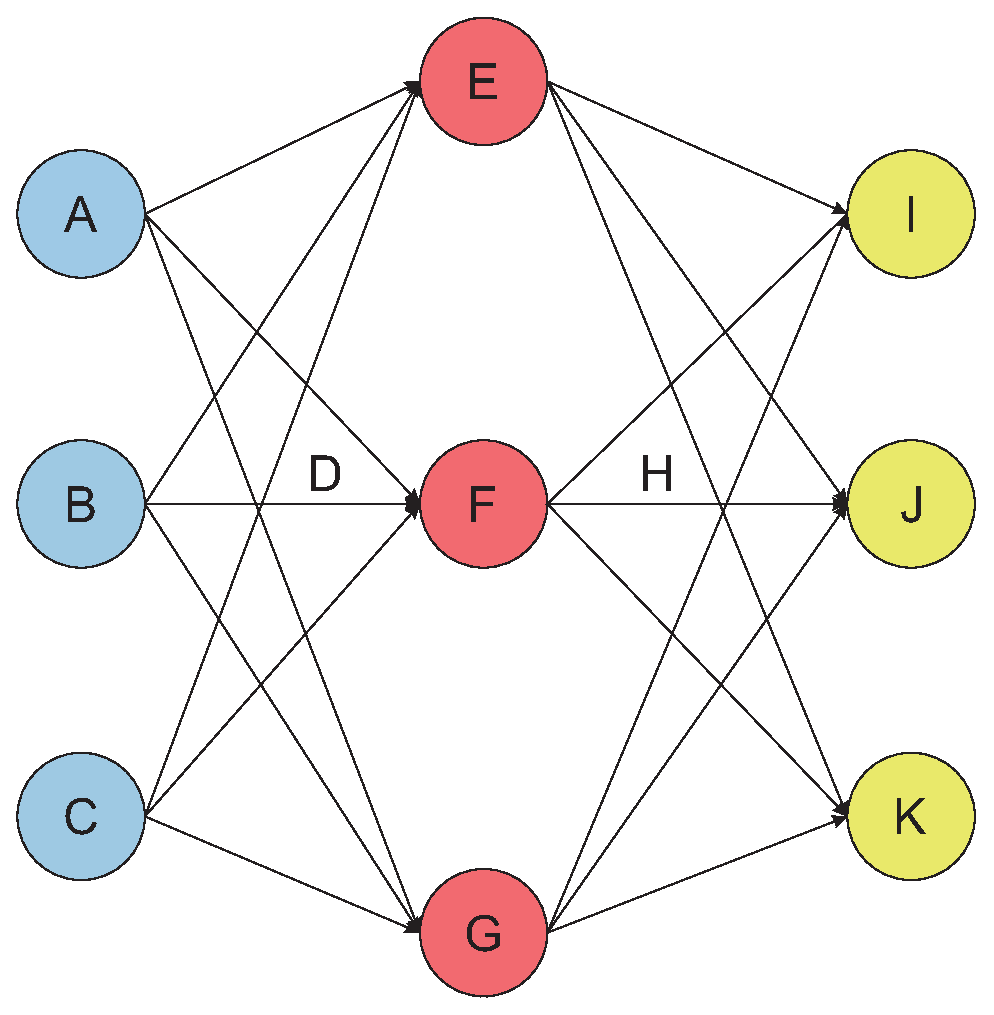
\includegraphics[scale=0.6]{images//11_2.eps}
\\~\\
\caption{Neural Network with single hidden layer}\label{NN}
\end{figure}

We denote the complete set of weights by $\boldsymbol{\theta}$, which consists of
\begin{equation*}
\boldsymbol{\theta} = 
\left\{
\begin{array}{l}
\boldsymbol{\alpha} \\
\boldsymbol{\beta} 
\end{array} \right.
\end{equation*}

Each of the $\alpha_{j}$ and $\beta_{k}$ is a subset vector of $\boldsymbol{\alpha}$ and $\boldsymbol{\beta}$,
\begin{equation*}
\boldsymbol{\alpha} = \big( \boldsymbol{\alpha}_{1} ~~ \boldsymbol{\alpha}_{j} ~~ \dots ~~ \boldsymbol{\alpha}_{H} \big) = 
\begin{blockarray}{ccccc}
  & \multicolumn{4}{c}{$j$}  \\
  & \boldsymbol{\alpha}_{1} & \boldsymbol{\alpha}_{2}  & \cdots & \boldsymbol{\alpha}_{H} \\
\begin{block}{c(cccc)}
\multirow{4}{*}{$i$} & \alpha_{11} & \alpha_{21} & \cdots & \alpha_{H1} \\
  					 & \alpha_{12} & \alpha_{22} & \cdots & \alpha_{H2} \\
			     	 & \vdots      & \vdots      & \ddots & \vdots  \\
				     & \alpha_{1D} & \alpha_{2D} & \cdots & \alpha_{HD} \\
\end{block}
\end{blockarray}
\end{equation*}

\begin{equation*}
\boldsymbol{\alpha}^{T} = 
\begin{blockarray}{ccccc}
  & \multicolumn{4}{c}{$i$}  \\
\begin{block}{c(cccc)}
\multirow{4}{*}{$j$} & \alpha_{11} & \alpha_{12} & \cdots & \alpha_{1D} \\
  					 & \alpha_{21} & \alpha_{22} & \cdots & \alpha_{2D} \\
			     	 & \vdots      & \vdots      & \ddots & \vdots  \\
				     & \alpha_{H1} & \alpha_{H2} & \cdots & \alpha_{HD} \\
\end{block}
\end{blockarray}
\end{equation*}

\begin{equation*}
\boldsymbol{\beta} = \big( \boldsymbol{\beta}_{1} ~~ \boldsymbol{\beta}_{k} ~~ \dots ~~ \boldsymbol{\beta}_{C} \big) = 
\begin{blockarray}{ccccc}
  & \multicolumn{4}{c}{$k$}  \\
  & \boldsymbol{\beta}_{1} & \boldsymbol{\beta}_{2}  & \cdots & \boldsymbol{\beta}_{C} \\
\begin{block}{c(cccc)}
\multirow{4}{*}{$j$}  & \beta_{11} & \beta_{21} & \cdots & \beta_{C1} \\
  			          & \beta_{12} & \beta_{22} & \cdots & \beta_{C2} \\
 		  			  & \vdots      & \vdots      & \ddots & \vdots  \\
			          & \beta_{1H} & \beta_{2H} & \cdots & \beta_{CH} \\
\end{block}
\end{blockarray}
\end{equation*}


\begin{equation*}
\boldsymbol{\beta}^{T} = 
\begin{blockarray}{ccccc}
  & \multicolumn{4}{c}{$j$}  \\
\begin{block}{c(cccc)}
\multirow{4}{*}{$k$}  & \beta_{11} & \beta_{12} & \cdots & \beta_{1H} \\
  			          & \beta_{21} & \beta_{22} & \cdots & \beta_{2H} \\
 		  			  & \vdots      & \vdots      & \ddots & \vdots  \\
			          & \beta_{K1} & \beta_{K2} & \cdots & \beta_{CH} \\
\end{block}
\end{blockarray}
\end{equation*}


We can write the overall model as follows:
\begin{equation*}
x_{n} \xrightarrow{\boldsymbol{\alpha}} \mathbf{a}_{n} \xrightarrow{g} \mathbf{z}_{n} \xrightarrow{\boldsymbol{\beta}} \mathbf{b}_{n} \xrightarrow{h} \hat{\mathbf{y}}_{n}
\end{equation*}

$x_{n}$ is a vector of length $D$ containing $D$ variables for the $n$th observation. That is,
\begin{gather}
x_{n} = \begin{pmatrix}
  x_{n1} \\
  x_{n2} \\
  \vdots \\
  x_{nD} 
 \end{pmatrix}
\end{gather}

In general, we have the following models extract from the overall model, 
\begin{align*}
a_{nj} &= \boldsymbol{\alpha}_{j}^{T} x_{n}, ~ j = 1, \dots, H \\
z_{nj} &= g(a_{nj}),            ~ j = 1, \dots, H \\
b_{nk} &= \boldsymbol{\beta}_{k}^{T} \mathbf{z}_{n},  ~ k = 1, \dots, C \\
\hat{y}_{nk} &= h(b_{nk}), ~ k=1,\dots, C
\end{align*}

From the above equations, it's not hard to see that $\hat{y}_{nk}$ consisted from a bunch of other functions, this can be interpreted as,
\begin{equation}
\hat{\mathbf{y}}_{n} = h(\mathbf{b}_{n}) = h(\boldsymbol{\beta}^{T} \mathbf{z}_{n}) = h(\boldsymbol{\beta}^{T} g( \mathbf{a}_{n})) = h(\boldsymbol{\beta}^{T} g(\boldsymbol{\alpha}^{T} x_{n}))
\end{equation}

Summarize the points above, $x_{n}$ is the $n$th observation, $\mathbf{a}_{n} = \boldsymbol{\alpha}^{T} x_{n}$ be the pre-synaptic hidden layer, and $\mathbf{z}_{n} = g( \mathbf{a}_{n})$ be the post-synaptic
hidden layer, where $g$ is some transfer funciton. We typically use $g(a)=sigm(a)$, but we may also use $g(a)=tanh(a)$. We now convert this hidden layer to the output layer. Let $\mathbf{b}_{n} = \boldsymbol{\beta}^{T} \mathbf{z}_{n}$ be the pre-synaptic output layer, and $\hat{\mathbf{y}}_{n}=h(\mathbf{b}_{n})$ be the post-synaptic output layer, where $h$ is another nonlinearity. 
For a regression model, we use $h(\mathbf{b})= \mathbf{b}$; for binary classification, we use $h(\mathbf{b})= [sigm(b_{1}),\dots,sigm(b_{c})]$; for multi-class classification, we use $h(\mathbf{b})= \mathcal{S}(\mathbf{b})$.


\subsection{Backpropagation neural networks}
We now discuss how to compute the gradient vector of the NLL(negative log likelihood) by applying the chain rule of calculus. The resulting algorithm is known as backpropagation.~\\

In the regression case, with $C$ outputs, the NLL is given by the by the squared error:
\begin{equation}
J(\boldsymbol{\theta}) = -\sum\limits_{n}\sum\limits_{k}(\hat{y}_{nk}(\boldsymbol{\theta})-y_{nk})^{2}
\end{equation}

In the classification case, with $C$ classes, the NLL is given by the cross entropy,
\begin{equation}
J(\boldsymbol{\theta}) = -\sum\limits_{n} \sum\limits_{k} y_{nk} \log \hat{y}_{nk}(\boldsymbol{\theta}) 
\end{equation}

Our task is to compute $\frac{d}{d\boldsymbol{\theta}}J$. The overall gradient is obtained by summing over $n$, we will derive this for each $n$ separately or we will perform mini-batch and summing the batch size.
Let us start by considering the output layer weights. We have
\begin{equation}
\nabla_{\boldsymbol{\beta}_{k}} J_{n} = \frac{\partial J_{n}}{\partial b_{nk}} \nabla_{\boldsymbol{\beta}_{k}} b_{nk} = \frac{\partial J_{n}}{\partial b_{nk}} \mathbf{z}_{n}
\end{equation}

Assuming $h$ is canonical link function for the output GLM, then 
\begin{equation}
\frac{\partial J_{n}}{\partial b_{nk}} = \delta^{\beta}_{nk} = (\hat{y}_{nk}-y_{nk})
\end{equation}

So the overall gradient is 
\begin{equation}
\nabla_{\boldsymbol{\beta}_{k}} J_{n} = \delta^{\beta}_{nk} \mathbf{z}_{n}
\end{equation}
which is the pre-synaptic input to the output layer, namely $\mathbf{z}_{n}$, times the error signal, namely $\delta^{\beta}_{nk}$.~\\

For the input layer weights, we have 
\begin{equation}
\nabla_{\boldsymbol{\alpha}_{j}} J_{n} = \frac{\partial J_{n}}{\partial a_{nj}} \nabla_{\boldsymbol{\alpha}_{j}} a_{nj} = \delta^{\alpha}_{nj} x_{n}
\end{equation}

The first level error signal $\delta^{\alpha}_{nj}$, 
\begin{equation}
\delta^{\alpha}_{nj} =  \frac{\partial J_{n}}{\partial a_{nj}} = \sum\limits_{k} \frac{\partial J_{n}}{\partial b_{nk}} \frac{\partial b_{nk}}{\partial a_{nj}}
\end{equation}

where,
\begin{equation}
\frac{\partial b_{nk}}{\partial a_{nj}} = \frac{\partial b_{nk}}{\partial z_{nj}} \frac{\partial z_{nj}}{\partial a_{nj}} = \beta_{kj} g'(a_{nj})
\end{equation}

So, the first level error signal $\delta^{\alpha}_{nj}$ is,
\begin{equation}
\delta^{\alpha}_{nj} =  \frac{\partial J_{n}}{\partial a_{nj}} = \sum\limits_{k} \delta^{\beta}_{nk} \beta_{kj} g'(a_{nj})
\end{equation}

In the end, the input layer weights looks like
\begin{equation}
\nabla_{\boldsymbol{\alpha}_{j}} J_{n} = \delta^{\alpha}_{nj} x_{n} = \sum\limits_{k} \delta^{\beta}_{nk} \beta_{kj} g'(a_{nj})x_{n}
\end{equation}

Given the derivatives, a gradient descent update at the $(r+1)$st iteration has the form
\begin{align*}
\boldsymbol{\beta}_{k}^{(r+1)} &=  \boldsymbol{\beta}_{k}^{(r)} - \eta \sum\limits_{n} \nabla_{\boldsymbol{\beta}_{k}} J_{n} \\
\boldsymbol{\alpha}_{j}^{(r+1)} &= \boldsymbol{\alpha}_{j}^{(r)} - \eta \sum\limits_{n} \nabla_{\boldsymbol{\alpha}_{j}} J_{n} 
\end{align*}

Learning can be carried out online - processing each observation one at a time, updating the gradient after each training case, and cycling through the training cases many times. 
In this case, the sums of $n$ in the update equations are replaced with single summation $k$. 
Online training allows the network to handle large training sets, and also update the weights as new observations come in.

The learning rate $\eta$ for batch learning is usually taken to be a constant, and can be optimized by a \textbf{line search}.

\subsubsection{Example 1}
\begin{figure}[H]
\centering
\psfrag{A}[c][c]{$x_{1}$}
\psfrag{B}[c][c]{$x_{2}$}
\psfrag{C}[c][c]{$z_{1}$}
\psfrag{D}[c][c]{$z_{2}$}
\psfrag{E}[c][c]{$z_{3}$}
\psfrag{F}[c][c]{$y_{1}$}
\psfrag{G}[c][c]{$y_{2}$}
\psfrag{a}[c][c]{\tiny $\alpha_{11}$}
\psfrag{b}[c][c]{\tiny $\alpha_{21}$}
\psfrag{c}[c][c]{\tiny $\alpha_{31}$}
\psfrag{d}[c][c]{\tiny $\alpha_{12}$}
\psfrag{e}[c][c]{\tiny $\alpha_{22}$}
\psfrag{f}[c][c]{\tiny $\alpha_{32}$}
\psfrag{g}[c][c]{\tiny $\beta_{11}$}
\psfrag{h}[c][c]{\tiny $\beta_{21}$}
\psfrag{i}[c][c]{\tiny $\beta_{12}$}
\psfrag{j}[c][c]{\tiny $\beta_{22}$}
\psfrag{k}[c][c]{\tiny $\beta_{13}$}
\psfrag{l}[c][c]{\tiny $\beta_{23}$}
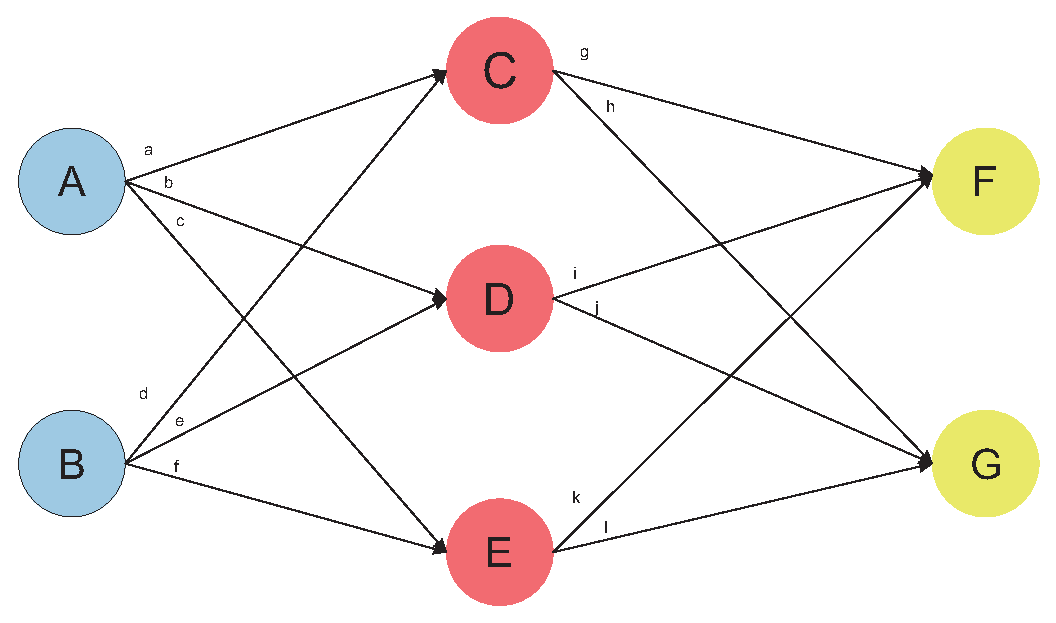
\includegraphics[scale=0.6]{images//example-1.eps}
\\~\\
\end{figure}

\begin{gather}
\boldsymbol{\alpha} = \begin{pmatrix}
 \boldsymbol{\alpha}_{1} & \boldsymbol{\alpha}_{2}  & \boldsymbol{\alpha}_{3}
 \end{pmatrix}
\end{gather}

\begin{gather}
\boldsymbol{\alpha}^{T} = \begin{pmatrix}
  \alpha_{11} & \alpha_{12}  \\
  \alpha_{21} & \alpha_{22}  \\
  \alpha_{31} & \alpha_{32}
 \end{pmatrix}
\end{gather}

\begin{gather}
\boldsymbol{\beta} = \begin{pmatrix}
 \boldsymbol{\beta}_{1} & \boldsymbol{\beta}_{2} 
 \end{pmatrix}
\end{gather}

\begin{gather}
\boldsymbol{\beta}^{T} = \begin{pmatrix}
  \beta_{11} & \beta_{12} & \beta_{13} \\
  \beta_{21} & \beta_{22} & \beta_{23}
 \end{pmatrix}
\end{gather}

The first output layer,
\begin{align*}
a_{1} &= \boldsymbol{\alpha}_{1}^{T} x = \sum\limits_{i=1}^{2} \alpha_{1i}x_{i}  \\
a_{2} &= \boldsymbol{\alpha}_{2}^{T} x = \sum\limits_{i=1}^{2} \alpha_{2i}x_{i} \\
a_{3} &= \boldsymbol{\alpha}_{3}^{T} x = \sum\limits_{i=1}^{2} \alpha_{3i}x_{i}
\end{align*}

So, 
\begin{gather}
\mathbf{a} = \begin{pmatrix}
  a_{1} \\
  a_{2} \\
  a_{3}
 \end{pmatrix}
\end{gather}

The post-synaptic hidden layer
\begin{gather}
\mathbf{z} = \begin{pmatrix}
  z_{1} \\
  z_{2} \\
  z_{3}
 \end{pmatrix} = \begin{pmatrix}
  g(a_{1}) \\
  g(a_{2}) \\
  g(a_{3})
 \end{pmatrix}
\end{gather}

The second output layer,
\begin{align*}
b_{1} &= \boldsymbol{\beta}_{1}^{T} \mathbf{z} = \sum\limits_{j=1}^{3} \beta_{1j}z_{j}  \\
b_{2} &= \boldsymbol{\beta}_{2}^{T} \mathbf{z} = \sum\limits_{j=1}^{3} \beta_{2j}z_{j}
\end{align*}

The estimated response,
\begin{gather*}
\mathbf{\hat{y}} = \begin{pmatrix}
  h(b_{1}) \\
  h(b_{2})
 \end{pmatrix} = \begin{pmatrix}
  \hat{y}_{1} \\
  \hat{y}_{2}
 \end{pmatrix}
\end{gather*}

a gradient descent update at the $(r+1)$st iteration has the form

\begin{equation*}
\boldsymbol{\beta}_{1}^{(r+1)} = \boldsymbol{\beta}_{1}^{(r)} - \eta \sum\limits_{n} \nabla_{\boldsymbol{\beta}_{1}} J_{n} = \begin{pmatrix}
  \beta_{11} \\
  \beta_{12} \\
  \beta_{13}
 \end{pmatrix} - \eta \left( \sum\limits_{n} (\hat{y}_{n1}-y_{n1})  \begin{pmatrix}
  z_{n1} \\
  z_{n2} \\
  z_{n3}
 \end{pmatrix} \right)
\end{equation*}

\begin{equation*}
\boldsymbol{\beta}_{2}^{(r+1)} = \boldsymbol{\beta}_{2}^{(r)} - \eta \sum\limits_{n} \nabla_{\boldsymbol{\beta}_{2}} J_{n} = \begin{pmatrix}
  \beta_{21} \\
  \beta_{22} \\
  \beta_{23}
 \end{pmatrix} - \eta \left( \sum\limits_{n} (\hat{y}_{n2}-y_{n2})  \begin{pmatrix}
  z_{n1} \\
  z_{n2} \\
  z_{n3}
 \end{pmatrix} \right)
\end{equation*}


\begin{equation*}
\boldsymbol{\alpha}_{1}^{(r+1)} = \boldsymbol{\alpha}_{1}^{(r)} - \eta \sum\limits_{n} \nabla_{\boldsymbol{\alpha}_{1}} J_{n} = \begin{pmatrix}
  \alpha_{11} \\
  \alpha_{12} \\
 \end{pmatrix} - \eta \left( \sum\limits_{n} \sum\limits_{k} (\delta_{nk}^{\beta} \beta_{k1})g'(a_{1}) \begin{pmatrix}
  x_{n1} \\
  x_{n2} 
 \end{pmatrix} \right)
\end{equation*}

\begin{equation*}
\boldsymbol{\alpha}_{2}^{(r+1)} = \boldsymbol{\alpha}_{2}^{(r)} - \eta \sum\limits_{n} \nabla_{\boldsymbol{\alpha}_{2}} J_{n} = \begin{pmatrix}
  \alpha_{21} \\
  \alpha_{22} \\
 \end{pmatrix} - \eta \left( \sum\limits_{n} \sum\limits_{k} (\delta_{nk}^{\beta} \beta_{k2})g'(a_{2}) \begin{pmatrix}
  x_{n1} \\
  x_{n2} 
 \end{pmatrix} \right)
\end{equation*}

\begin{equation*}
\boldsymbol{\alpha}_{3}^{(r+1)} = \boldsymbol{\alpha}_{3}^{(r)} - \eta \sum\limits_{n} \nabla_{\boldsymbol{\alpha}_{3}} J_{n} = \begin{pmatrix}
  \alpha_{31} \\
  \alpha_{32} \\
 \end{pmatrix} - \eta \left( \sum\limits_{n} \sum\limits_{k} (\delta_{nk}^{\beta} \beta_{k3})g'(a_{3}) \begin{pmatrix}
  x_{n1} \\
  x_{n2} 
 \end{pmatrix} \right)
\end{equation*}

The graph of back propagation
\begin{figure}[H]
\centering
\psfrag{A}[c][c]{$x_{1}$}
\psfrag{B}[c][c]{$x_{2}$}
\psfrag{C}[c][c]{$z_{1}$}
\psfrag{D}[c][c]{$z_{2}$}
\psfrag{E}[c][c]{$z_{3}$}
\psfrag{F}[c][c]{$y_{1}$}
\psfrag{G}[c][c]{$y_{2}$}
\psfrag{a}[c][c]{\color{red} \tiny $\alpha_{11}- \delta^{\alpha}_{1} x_{1} $}
\psfrag{b}[c][c]{\color{red} \tiny $\alpha_{12}- \delta^{\alpha}_{1} x_{2} $}
\psfrag{c}[c][c]{\color{blue} \tiny $\alpha_{21}- \delta^{\alpha}_{2}x_{1}$}
\psfrag{d}[c][c]{\color{blue} \tiny $\alpha_{22}- \delta^{\alpha}_{2}x_{2}$}
\psfrag{e}[c][c]{\tiny $\alpha_{31}- \delta^{\alpha}_{3}x_{1}$}
\psfrag{f}[c][c]{\tiny $\alpha_{32}- \delta^{\alpha}_{3}x_{2}$}
\psfrag{g}[c][c]{\tiny $\beta_{11} - \delta^{\beta}_{1} z_{1}$}
\psfrag{h}[c][c]{\tiny $\beta_{12} - \delta^{\beta}_{1} z_{2}$}
\psfrag{i}[c][c]{\tiny $\beta_{13} - \delta^{\beta}_{1} z_{3}$}
\psfrag{j}[c][c]{\tiny $\beta_{21} - \delta^{\beta}_{2} z_{1}$}
\psfrag{k}[c][c]{\tiny $\beta_{22} - \delta^{\beta}_{2} z_{2}$$}
\psfrag{l}[c][c]{\tiny $\beta_{23} - \delta^{\beta}_{2} z_{3}$}
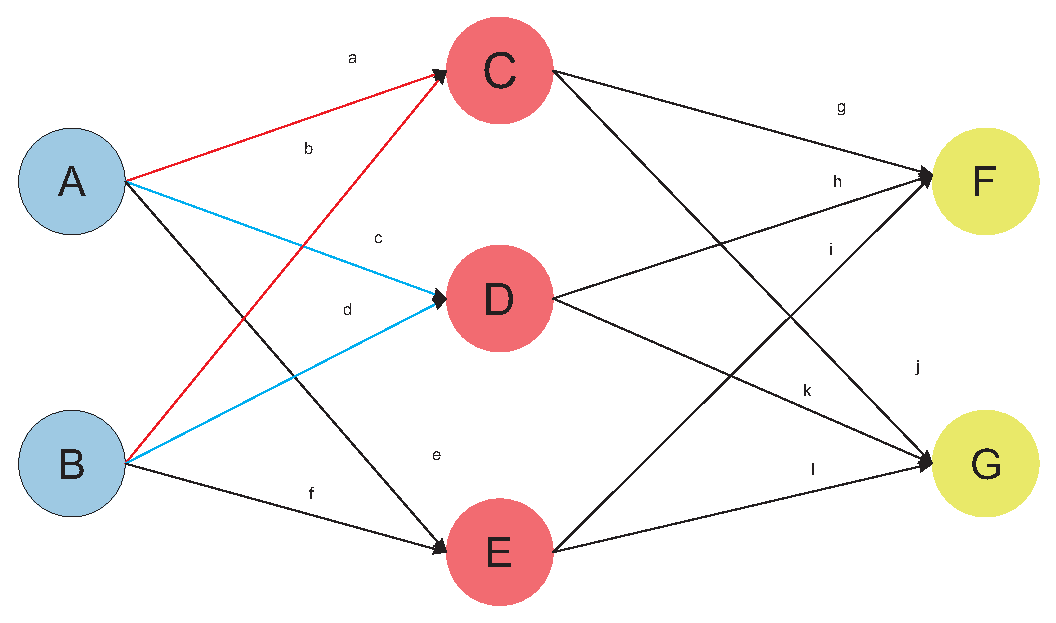
\includegraphics[scale=0.6]{images//example-1_back.eps}
\\~\\
\end{figure}

I didn't add learning rate on the update, since the tag is too small to add any words on it.

\subsection{General form of Feed-forward and Back-propagation}

\subsubsection{Notation}
\begin{itemize}
\item $\overrightarrow{X}_{\ell}$ : denotes the input data matrix in layer $\ell$ with $N$ input size and $D$ input dimensional size.  
\item $\overrightarrow{W}_{\ell}$ : denotes the weight matrix in layer $\ell$ with $D$ input dimensional size and $H$ output layer size.
\item $\vec{b}_{\ell}$ : denotes the bias vector in layer $\ell$ with $H$ output layer size.
\item $\overrightarrow{a}_{\ell}$ : denotes the output matrix before activation from layer $\ell$.
\item $f_{\ell}(\cdot)$ : denotes the activation function in layer $\ell$. 
\end{itemize}

\begin{equation*}
\overrightarrow{X}_{\ell} =  \begin{blockarray}{cccc}
                                     & \multicolumn{3}{c}{$D$}  \\
\begin{block}{c(ccc)}
\multirow{3}{*}{$N$} &    &       &    \\
  					                 &      &  \prescript{n}{}{(x_{\ell})}_{d}     &     \\
			     	                 &      &       &       \\
\end{block}
\end{blockarray}
\end{equation*}

\begin{equation*}
\overrightarrow{W}_{\ell} =  \begin{blockarray}{cccc}
                                     & \multicolumn{3}{c}{$H$}  \\
\begin{block}{c(ccc)}
\multirow{3}{*}{$D$} &    &       &    \\
  					                 &      &  {(w_{\ell})}^{d}_{h}     &     \\
			     	                 &      &       &       \\
\end{block}
\end{blockarray}
\end{equation*}

\begin{equation*}
\vec{b}_{\ell} =  \begin{blockarray}{ccc}
    \multicolumn{3}{c}{$H$}  \\
\begin{block}{(ccc)}
    &    {(b_{\ell})}_{h}     &    \\
\end{block}
\end{blockarray}
\end{equation*}

\begin{equation*}
\overrightarrow{a}_{\ell} =  \begin{blockarray}{cccc}
                                     & \multicolumn{3}{c}{$H$}  \\
\begin{block}{c(ccc)}
\multirow{3}{*}{$N$} &    &       &    \\
  					                 &      & \prescript{n}{}{(a_{\ell})}_{h} =  \prescript{n}{}{(x_{\ell})}_{d} \cdot {(w_{\ell-1})}^{d}_{h}  + (b_{\ell-1})_{h}    &     \\
			     	                 &      &       &       \\
\end{block}
\end{blockarray}
\end{equation*}

\begin{equation}
\overrightarrow{X}_{\ell+1} = f_{\ell}(\overrightarrow{a}_{\ell} )
\end{equation}

\subsubsubsection{Feed-Forward Neural Network}

For a two layer fully-connected neural network ,  the network has the following architecture: 
\begin{equation}
\footnotesize
\overrightarrow{X}_{\ell-1} \mapsto \overrightarrow{a}_{\ell-1} = \overrightarrow{X}_{\ell-1} \overrightarrow{W}_{\ell-2} \rightarrow 
\overrightarrow{X}_{\ell} = f_{\ell-1}(\overrightarrow{a}_{\ell-1}) \mapsto \overrightarrow{a}_{\ell} = \overrightarrow{X}_{\ell} \overrightarrow{W}_{\ell-1} \rightarrow \hat{y} = \text{softmax}(\overrightarrow{a}_{\ell})
\end{equation}

We denote the loss function as,
\begin{equation}
L = loss(y, \hat{y}) = \sum\limits_{n} \sum\limits_{h} loss(\prescript{n}{}{y_{h}}, \prescript{n}{}{\hat{y}}_{h})
\end{equation}

\subsubsubsection{Back-propagation Neural Network}
Let us start by considering the last layer weights ${(w_{\ell-1})}^{d}_{h} $ and perform the derivative on the loss function
\begin{equation}
\frac{\partial}{\partial {(w_{\ell-1})}^{d}_{h}} L = \frac{\partial L}{\partial \prescript{n}{}{(a_{\ell})}_{h}} \frac{\partial \prescript{n}{}{(a_{\ell})}_{h}}{\partial {(w_{\ell-1})}^{d}_{h}} = \frac{\partial L}{\partial \prescript{n}{}{(a_{\ell})}_{h}}  \prescript{n}{}{(x_{\ell})}_{d} =  \prescript{n}{}{(\delta_{\ell})}_{h} \cdot \prescript{n}{}{(x_{\ell})}_{d} = \prescript{}{n}{(x_{\ell}^{T})}^{d} \cdot \prescript{n}{}{(\delta_{\ell})}_{h} 
\end{equation}

For the ease of notation,  we denote  $\prescript{n}{}{(\delta_{\ell})}_{h}$ as the error signal in layer $\ell$. Now, we derivative of ${(w_{\ell-2})}^{d}_{h}$ on the loss function, 
\begin{align}
\frac{\partial}{\partial {(w_{\ell-2})}^{d}_{h}} L  &=  \frac{\partial L}{\partial \prescript{n}{}{(a_{\ell-1})}_{h}} \frac{\partial \prescript{n}{}{(a_{\ell-1})}_{h}}{\partial {(w_{\ell-2})}^{d}_{h}} \\
& = \frac{\partial L}{\partial \prescript{n}{}{(a_{\ell-1})}_{h}}  \prescript{n}{}{(x_{\ell-1})}_{d} \\
& = \prescript{}{n}{(x_{\ell-1}^{T})}^{d} \cdot \prescript{n}{}{(\delta_{\ell-1})}_{h} 
\end{align}


For a two layer($\ell = 2$) fully connected neural network,  the error signal for the last layer has the below form,
\begin{align}
\begin{split}
\prescript{n}{}{(\delta_{\ell})}_{h} &= \frac{\partial L}{\partial \prescript{n}{}{(a_{\ell})}_{h}} \\
															  &= loss'(y,\hat{y}) \hat{y}' \\
															  &= loss'(y,\hat{y}) \odot f'_{\ell}(\prescript{n}{}{(a_{\ell})}_{h})
\end{split}
\end{align}

For the error signal in the first layer,
\begin{align*}
\begin{split}
\prescript{n}{}{(\delta_{\ell-1})}_{h} &= \frac{\partial L}{\partial \prescript{n}{}{(a_{\ell-1})}_{h}} \\
																  &= \sum\limits_{d} \frac{\partial L}{\partial \prescript{n}{}{(a_{\ell})}_{d}} \cdot \frac{\partial \prescript{n}{}{(a_{\ell})}_{d}}{\partial \prescript{n}{}{(a_{\ell-1})}_{h}} \\
														          &= \sum\limits_{d} 	\prescript{n}{}{(\delta_{\ell})}_{d} \cdot \frac{\partial \prescript{n}{}{(a_{\ell})}_{d}}{\partial \prescript{n}{}{(a_{\ell-1})}_{h}}			  
\end{split}
\label{delta1}
\end{align*}

We'll show how to proof $\frac{\partial \prescript{n}{}{(a_{\ell})}_{d}}{\partial \prescript{n}{}{(a_{\ell-1})}_{h}}$. For $ \prescript{n}{}{(a_{\ell})}_{d}   $, we know that 
\begin{align*}
\prescript{n}{}{(a_{\ell})}_{d} &= \prescript{n}{}{(x_{\ell})}_{h} \cdot {(w_{\ell-1})}^{h}_{d}  + (b_{\ell-1})_{d} \\
													  &= f_{\ell-1}(\prescript{n}{}{(a_{\ell-1})}_{h}) {(w_{\ell-1})}^{h}_{d} + (b_{\ell-1})_{d}
\end{align*}
So,
\begin{equation}
\frac{\partial \prescript{n}{}{(a_{\ell})}_{d}}{\partial \prescript{n}{}{(a_{\ell-1})}_{h}} = f'_{\ell-1}(\prescript{n}{}{(a_{\ell-1})}_{h}) {(w_{\ell-1})}^{h}_{d} 
\end{equation}

Finally, the complete form of the error signal in the first layer,
\begin{align*}
\prescript{n}{}{(\delta_{\ell-1})}_{h} &= f'_{\ell-1}(\prescript{n}{}{(a_{\ell-1})}_{h}) \sum\limits_{d} 	\prescript{n}{}{(\delta_{\ell})}_{d} \cdot  {(w_{\ell})}^{h}_{d} \\
																  &= f'_{\ell-1}(\prescript{n}{}{(a_{\ell-1})}_{h}) \odot \prescript{n}{}{(\delta_{\ell})}_{d} \cdot {(w_{\ell}^{T})}^{d}_{h}
\end{align*}

The gradient of bias is similar with the above proof,
\begin{align*}
\frac{\partial}{\partial {(b_{\ell})}_{h}} L  &= \frac{\partial L}{\partial \prescript{n}{}{(a_{\ell})}_{h}} \frac{\partial \prescript{n}{}{(a_{\ell})}_{h}}{\partial {(b_{\ell})}_{h}} = \sum\limits_{n} \prescript{n}{}{(\delta_{\ell})}_{h} \\
\frac{\partial}{\partial {(b_{\ell-1})}_{h}} L  &= \frac{\partial L}{\partial \prescript{n}{}{(a_{\ell-1})}_{h}} \frac{\partial \prescript{n}{}{(a_{\ell-1})}_{h}}{\partial {(b_{\ell-1})}_{h}} = \sum\limits_{n} \prescript{n}{}{(\delta_{\ell-1})}_{h}
\end{align*}

The loss function, full gradients and L2 regularization, 
\begin{align*}
 L &= loss({y}, {\hat{y}}) + \frac{\lambda}{2} ( \overrightarrow{W}_\ell^2 + \overrightarrow{W}_{\ell-1}^2 ) \\
\frac{\partial}{\partial {(w_{\ell})}^{d}_{h}} L &= \prescript{}{n}{(x_{\ell}^{T})}^{d} \cdot \prescript{n}{}{(\delta_{\ell})}_{h} + \lambda {(w_{\ell})}^{d}_{h} \\
																				  &= \prescript{}{n}{(x_{\ell}^{T})}^{d} (loss'(y,\hat{y}) \odot f'_{\ell}(\prescript{n}{}{(a_{\ell})}_{h})) + \lambda {(w_{\ell})}^{d}_{h} \\
\frac{\partial}{\partial {(w_{\ell-1})}^{d}_{h}} L &= \prescript{}{n}{(x_{\ell-1}^{T})}^{d} \prescript{n}{}{(\delta_{\ell})}_{h} + \lambda {(w_{\ell-1})}^{d}_{h} \\
																					 &= \prescript{}{n}{(x_{\ell-1}^{T})}^{d} \cdot  (f'_{\ell-1}(\prescript{n}{}{(a_{\ell-1})}_{h}) \odot (\prescript{n}{}{(\delta_{\ell})}_{d} \cdot {(w_{\ell}^{T})}^{d}_{h})) + \lambda {(w_{\ell-1})}^{d}_{h} \\
\frac{\partial}{\partial {(b_{\ell})}_{h}} L  &= \frac{\partial L}{\partial \prescript{n}{}{(a_{\ell})}_{h}} \frac{\partial \prescript{n}{}{(a_{\ell})}_{h}}{\partial {(b_{\ell})}_{h}} = \sum\limits_{n} \prescript{n}{}{(\delta_{\ell})}_{h} \\
\frac{\partial}{\partial {(b_{\ell-1})}_{h}} L  &= \frac{\partial L}{\partial \prescript{n}{}{(a_{\ell-1})}_{h}} \frac{\partial \prescript{n}{}{(a_{\ell-1})}_{h}}{\partial {(b_{\ell-1})}_{h}} = \sum\limits_{n} \prescript{n}{}{(\delta_{\ell-1})}_{h}
\end{align*} 


\end{document}
